\documentclass[10pt]{scrartcl}
\usepackage[utf8]{inputenc}
\usepackage{lmodern}
\usepackage{amsmath, amssymb}
\usepackage{a4wide}
\usepackage{placeins}
\usepackage{graphicx}
\usepackage{hyperref}
\hypersetup{
    colorlinks,
    linkcolor   = blue,
    urlcolor    = blue,
    citecolor   = blue,
    anchorcolor = blue
}

%opening
\title{
Tuner \\
{\small frequency analysis of the microphone input suitable to tune instruments}
}
\author{by Richard Hartmann}

\renewcommand{\i}{\mathrm{i}}
\newcommand*{\defeq}{\mathrel{\vcenter{\baselineskip0.5ex \lineskiplimit0pt
                     \hbox{\scriptsize.}\hbox{\scriptsize.}}}=}
\newcommand*{\eqdef}{=\mathrel{\vcenter{\baselineskip0.5ex \lineskiplimit0pt
                     \hbox{\scriptsize.}\hbox{\scriptsize.}}}}
                     
\newcommand{\kll}[1]{\textit{#1}{,}{,}}
\newcommand{\kl}[1]{\textit{#1}{,}}
\renewcommand{\k}[1]{\textit{#1}}
\newcommand{\kh}[1]{\textit{#1}{'}}
\newcommand{\khh}[1]{\textit{#1}{'}{'}}
\newcommand{\khhh}[1]{\textit{#1}{'}{'}{'}}
\newcommand{\khhhh}[1]{\textit{#1}{'}{'}{'}{'}}
\newcommand{\khhhhh}[1]{\textit{#1}{'}{'}{'}{'}{'}}

\begin{document}

\maketitle
\newpage

\tableofcontents
\newpage

\section{Theory}

\subsection{Piano Keys -- Well-Tempered Tuning}

Starting at some reference key, e.g. the key \k{a} with a frequency of 440Hz, the key an octave higher has twice that frequency. 
Thus, the key an octave lower, half the frequency.
In twelve-tone equal temperament an octave is made up of twelve steps with frequencies that are equally spaced in a logarithmic scale.
So the frequency of the key, labeled in steps above/below the reference key \k{a} at frequency  440Hz is given by
\begin{equation}
    f_i = 2^{i/12} 440 \mathrm{Hz} \; .
\end{equation}
On a standard piano with 88 keys the reference key \k{a} is the 49th key.
So labeling the key with index $n$ from low to high yields the alternative expression
\begin{equation}
    f_n = 2^{(n-49)/12} 440 \mathrm{Hz} \; .
\end{equation}

This means, that the lowest key, i.e. the \kll{a} has a frequency of $f_1 = 27.5$Hz which amount to a period of $T_1 = 1/f_1 = 36.4\mathrm{ms}$. 
For the highest key \khhhh{c} it follows $f_{88} = 4186$Hz and $T = 0.239\mathrm{ms}$.


\subsection{Determine Frequency}

The task is to determine the base frequency contained in the recorded signal of the sound of a single key (single string).
We assume that the recoded signal is a super position of higher harmonics of the base frequency with possible phase shifts, 
\begin{equation}
    s(t) = \sum_{n=1}^N a_n \cos(\omega_n t + \phi_n)  \quad \text{with} \quad \omega_n = n \omega_0 \; .
    \label{eqn:model_input_signal}
\end{equation}
Of course, the amplitudes decay with time.
For a real time analysis, where short intervals of the input signal can be used only, we assume the amplitudes to be constant over such intervals.
If sufficiently many oscillations are contained, the Fourier integral shows maxima at the frequencies $\omega_n$.
Otherwise, the maxima are not consistent with the actual frequencies.
In that case, the base frequency can be determined by fitting the model (Eq. \eqref{eqn:model_input_signal}) to the input signal.
See Fig. \ref{fig:freq_recov} for a first example.

\begin{figure}[htb]
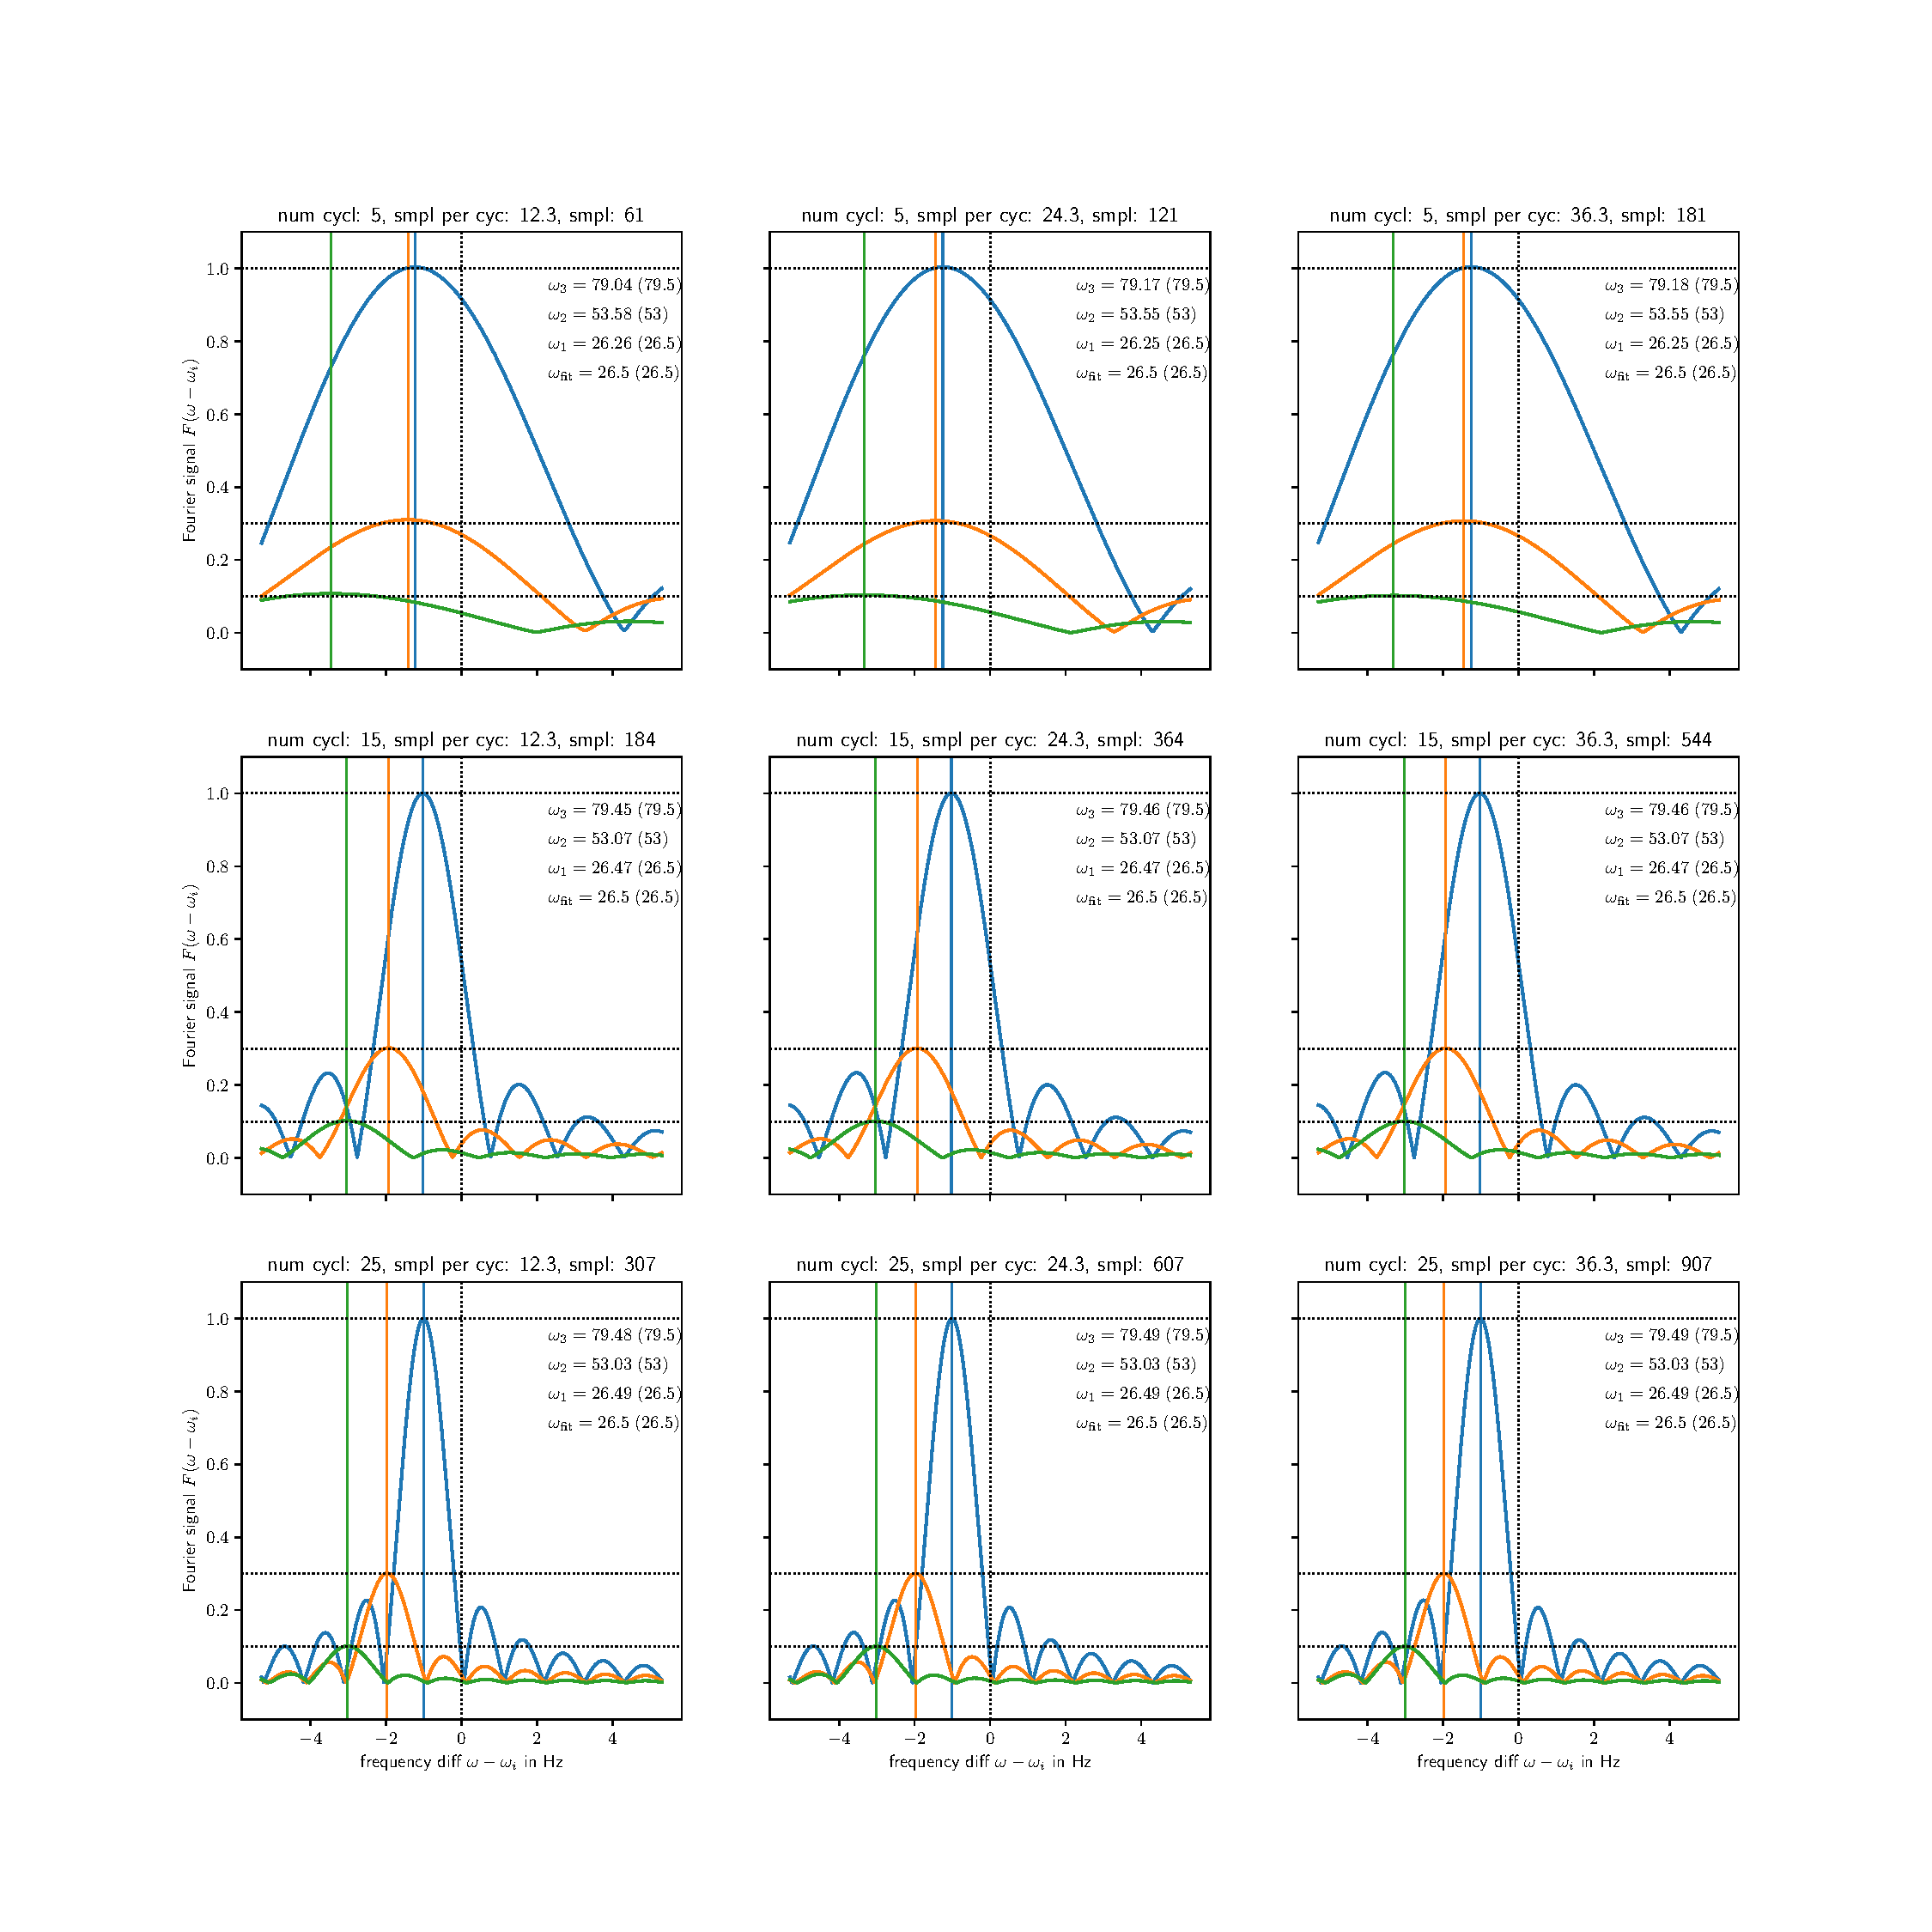
\includegraphics[width=\textwidth]{freq_recov}
\label{fig:freq_recov}
\caption{
The finite Fourier integral approximation of some input signal using a finite number of sampling pontes is shown.
The axes are such we expect a base frequency of $27.5$Hz (we want to tune the key to $27.5$Hz).
As test case, the signal we analyze is slightly detuned.
It has a base frequency of $26.5$Hz and higher harmonics contribution of $53$Hz and $79.5$Hz.
Note that the frequency axes is shifted for each higher harmonic by its expected value, i.e. $27.5$Hz, $2\cdot27.5$Hz and $3\cdot27.5$Hz.
In that way the frequency axes refers to the detuning.
For a perfectly tuned key and a trustworthy Fourier analysis, all maxima should align at zero.
In the first row, the input time interval contains 5 cycle of the base oscillation, with increasing number of sampling point from left to right.
In any case the maxima do not match the actual frequency of the test signal.
For larger time intervals of the input signal (top to bottom), the maxima agree with the actual frequency.
We conclude that 15 cycle with a sampling rate of 12.3 samples per cycle suffice to yield a good visual impression of the contained frequencies.
For a precise value of the base frequency, the model is fitted to the input signal, where the Fourier analysis is used to get useful the initial conditions for the least square minimization.
}
\end{figure}






\end{document}
